%%%%%%%%%%%%%%%%%%%%%%%%%%%%%%%%%%%%%%%%%
% baposter Landscape Poster
% LaTeX Template
% Version 1.0 (11/06/13)
%
% baposter Class Created by:
% Brian Amberg (baposter@brian-amberg.de)
%
% This template has been downloaded from:
% http://www.LaTeXTemplates.com
%
% License:
% CC BY-NC-SA 3.0 (http://creativecommons.org/licenses/by-nc-sa/3.0/)
%
%%%%%%%%%%%%%%%%%%%%%%%%%%%%%%%%%%%%%%%%%

%----------------------------------------------------------------------------------------
%	PACKAGES AND OTHER DOCUMENT CONFIGURATIONS
%----------------------------------------------------------------------------------------

\documentclass[potrait,paperwidth=20in,paperheight=30in,margin=1.5in,fontscale = 0.5]{baposter} % Adjust the font scale/size here

\usepackage{graphicx} % Required for including images
\usepackage{graphbox}
% \graphicspath{{figures/}} % Directory in which figures are stored
\usepackage{color}
\usepackage{amsmath} % For typesetting math
\usepackage{amssymb} % Adds new symbols to be used in math mode
\usepackage{amsthm,thmtools}
\usepackage{framed}
\usepackage{booktabs} % Top and bottom rules for tables
\usepackage{enumitem} % Used to reduce itemize/enumerate spacing
\usepackage{palatino} % Use the Palatino font
\usepackage[font=small,labelfont=bf]{caption} % Required for specifying captions to tables and figures
\usepackage{nicefrac}

\usepackage{mathtools}
\usepackage{bm}

\usepackage{tabularx}

\usepackage{multicol} % Required for multiple columns
\setlength{\columnsep}{1.5em} % Slightly increase the space between columns
\setlength{\columnseprule}{0mm} % No horizontal rule between columns

\usepackage{etoolbox}
\patchcmd{\thebibliography}{\section*{\refname}}{}{}{}

\usepackage{tikz} % Required for flow chart
\usetikzlibrary{shapes,arrows} % Tikz libraries required for the flow chart in the template
\usetikzlibrary{scopes}
\usetikzlibrary{shapes.misc}
\tikzset{cross/.style={cross out, draw=black, minimum size=2*(#1-\pgflinewidth), inner sep=0pt, outer sep=0pt},
%default radius will be 1pt.
  cross/.default={2pt}}
\newcommand{\mygrid}{%
    \draw[black,thin,xstep=0.05,ystep=0.05] (0,0) grid (1,1);
    \draw[black,thick,xstep=0.1,ystep=0.1] (0,0) grid (1,1);
}

% \usepackage{wrapfig}
\usepackage{float}
% \usepackage{subcaption}
% \usepackage{epstopdf}

\newcommand{\compresslist}{ % Define a command to reduce spacing within itemize/enumerate environments, this is used right after \begin{itemize} or \begin{enumerate}
\setlength{\itemsep}{1pt}
\setlength{\parskip}{0pt}
\setlength{\parsep}{0pt}
}

\definecolor{lightblue}{rgb}{0.145,0.6666,1} % Defines the color used for content box headers
\definecolor{cmured}{RGB}{143,1,31} % Defines the color used for content box headers

\DeclareMathOperator{\conv}{\text{conv}}

% \declaretheoremstyle[
%   headfont=\kern-2.5em\bfseries,
%   bodyfont=\normalfont,
%   headindent=0pt,
% ]{INDENTthm}
% \declaretheorem[
%   within=section,
%   style=INDENTthm,
%   name=Theorem
% ]{thm}

% \usepackage{etoolbox}
% \makeatletter
% \AtBeginEnvironment{thm}{%
%   \patchcmd\@thm
%     {\trivlist}
%     {\list{}{\leftmargin2.5em\itemindent-15em}}
%     {}{}%
%   \patchcmd\thmt@original@endthm{\endtrivlist}{\endlist}{}{}%
% }
% \makeatother

% \makeatletter
% \def\@begintheorem#1#2{\trivlist
% \item[\hskip \labelsep{\bfseries #1\ #2}]\mbox\newline\quote\itshape}
% \def\@opargbegintheorem#1#2#3{\trivlist
% \item[\hskip \labelsep{\bfseries #1\ #2\ (#3)}]\mbox\newline\quote\itshape}
% \def\@endtheorem{\endquote\endtrivlist}
% \makeatother
\newtheorem{theorem}{Thm}

\begin{document}

\begin{poster}
{
  columns=2,
  headerborder=closed, % Adds a border around the header of content boxes
  colspacing=1em, % Column spacing
  bgColorOne=white, % Background color for the gradient on the left side of the poster
  bgColorTwo=white, % Background color for the gradient on the right side of the poster
  borderColor=black, % Border color
  headerColorOne=black, % Background color for the header in the content boxes (left side)
  headerColorTwo=cmured,%red, % Background color for the header in the content boxes (right side)
  headerFontColor=white, % Text color for the header text in the content boxes
  boxColorOne=white, % Background color of the content boxes
  textborder=roundedleft, % Format of the border around content boxes, can be: none, bars, coils, triangles, rectangle, rounded, roundedsmall, roundedright or faded
  eyecatcher=true, % Set to false for ignoring the left logo in the title and move the title left
  headerheight=0.1\textheight, % Height of the header
  headershape=roundedright, % Specify the rounded corner in the content box headers, can be: rectangle, small-rounded, roundedright, roundedleft or rounded
  headerfont=\large\bf\textsc, % Large, bold and sans serif font in the headers of content boxes
  % textfont={\setlength{\parindent}{1.5em}}, % Uncomment for paragraph indentation
  linewidth=2pt % Width of the border lines around content boxes
}
%----------------------------------------------------------------------------------------
%	TITLE SECTION 
%----------------------------------------------------------------------------------------
%
{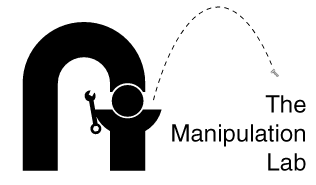
\includegraphics[height=6em]{images/mlab_logo.png}} % Second university/lab logo on the right
{\Huge\textbf{Exact Bounds on the Contact Driven \\Motion of a Sliding
    Object,\\\vspace{1mm} With Applications to Robotic Pulling}
  \vspace{3mm}} % Poster title
  {{{Eric Huang, Ankit Bhatia, Byron Boots, and Matthew
      T. Mason}}\vspace{3mm}} % Author names and institution
{
\includegraphics[height=6em]{images/ri_logo.png}} % First university/lab logo on the left
\headerbox{Abstract}{name=ab,column=0,row=0}{ This work explores the
  \textbf{quasi-static motion of a planar slider being pushed or pulled
  through a single contact}. Our main contributions are
  \begin{itemize}
  \item A method for computing \textbf{exact angular velocity bounds} on the
    object motion,
  \item A method that uses the bounds to \textbf{plan robotic pulling
    trajectories} that \textbf{guarantee convergence} to the target
    pose.
  \end{itemize}
}
\headerbox{Related Work}{name=rw,column=0,below=ab}{
  \begin{itemize}
  \item All prior motion bounds such as Peshkin, Bisector, VStrip are
    \textbf{inexact} \cite{Mason}.
  \item Robotic pulling has been \textbf{under explored}, limited to
    orienting asymmetrical convex polygons
    \cite{berretty2001orienting}.
  \end{itemize}
}
\headerbox{Background}{name=bg,column=0,below=rw}{
  
  Let the following diagram be our pulling reference frame. 
  \begin{center}
    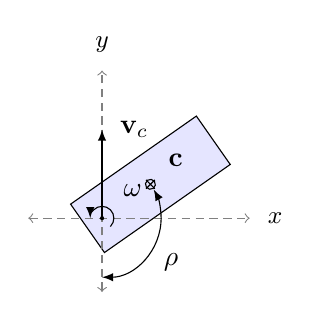
\begin{tikzpicture}
      [
      scale=0.75, every node/.style={scale=1},
      force/.style={>=latex,draw=black,fill=black},
      axis/.style={densely dashed,draw=gray,font=\small},
      ]
      \def\iangle{35} % Angle of the inclined plane
      \fill[draw=black,fill=blue!10,thin,rotate=\iangle] (-0.3,-0.5) rectangle (2.3,.5);
      \draw[rotate=\iangle] (1,0) circle[radius=2.4pt] node[cross] {};
      \draw[rotate=\iangle] (1,0) node[above right=3pt] {$\mathbf{c}$};
      {[axis,<->]
        \draw (-1.25,0) -- (2.5,0) node[right=3pt] {$x$};
        \draw (0,-1.25) -- (0,2.5) node[above=3pt] {$y$};
      }
      {[force,->]
        \draw (0,0) -- ++(0,1.5) node[right=3pt] {$\mathbf{v}_c$};
      }
      \def\ilen{1}
      {
        % \draw[rotate=\iangle,style=densely dashed] (0,0) -- (\ilen,0);
        \draw[rotate=-90,style=<->,>=latex] ++(\ilen,0) arc (0:90+\iangle-6:\ilen);
        \draw[rotate=-45] (\ilen+0.05,0) node[right=3pt] {$\rho$};
      }
      \def\wlen{0.2}
      {
        % \draw[rotate=\iangle,style=densely dashed] (0,0) -- (\ilen,0);
        \draw[rotate=-45,style=->,>=latex] ++(\wlen,0) arc (0:225:\wlen);
        \draw[rotate=45] (\wlen-0.05,0) node[above right=2pt] {$\omega$};
      }
      \fill (0,0) circle [radius=1.pt];
      % \fill (1.8,0) circle [radius=1.pt] node[below right] {$\mathbf{r_c}$};
    \end{tikzpicture}
  \end{center}

  The \textbf{quasi-static motion model} implies that there is
  \textbf{zero moment} at the contact point (origin)
  \begin{equation}
    \mathbf{m}_f = -\mu\int_{R}\mathbf{r}\times\frac{\mathbf{v}(\mathbf{r})}{\lVert\mathbf{v}(\mathbf{r})\rVert} p(\mathbf{r}) dA = 0. \label{eq:moment-at-contact}
  \end{equation}

  For a given twist, the \textbf{moment envelope} is the set of all
  feasible centers of pressure and total frictional moments,
  i.e. generated by some pressure distribution.\\

  It is also the \textbf{convex hull} of the \textbf{unit-moment
    surface}
  \begin{equation}
    G(\mathbf{x}) =
    \begin{bmatrix*}
      \mathbf{x}\\
      -\mu \mathbf{x}\times\frac{\mathbf{v}(\mathbf{x})}{\lVert\mathbf{v}(\mathbf{x})\rVert}
    \end{bmatrix*} \label{eq:moment-surface-function}
  \end{equation}
%   \begin{equation}
%     g(\mathbf{x}) = -\mu f_0\,\mathbf{x}\times \frac{A(\mathbf{x})\mathbf{v}^+}{\lVert A(\mathbf{x})\mathbf{v}^+ \rVert} \label{eq:unit-moment-at-x}
%   \end{equation}

  \begin{center}
  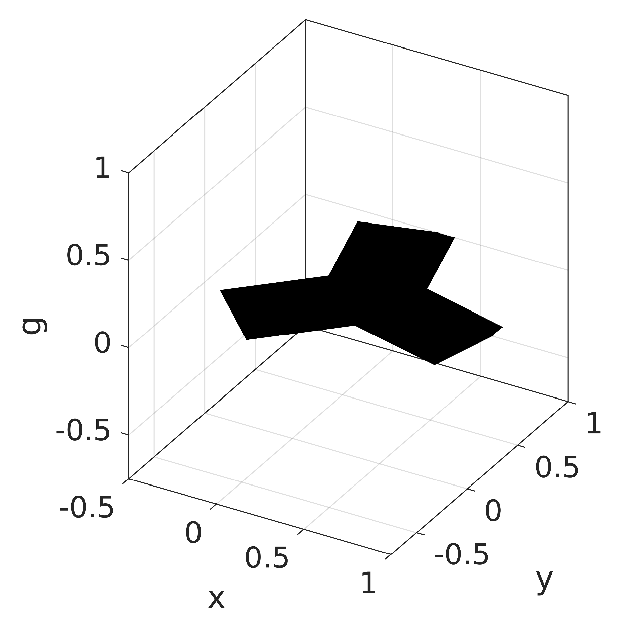
\includegraphics[width=0.24\columnwidth]{fig/moment_hull_1}
  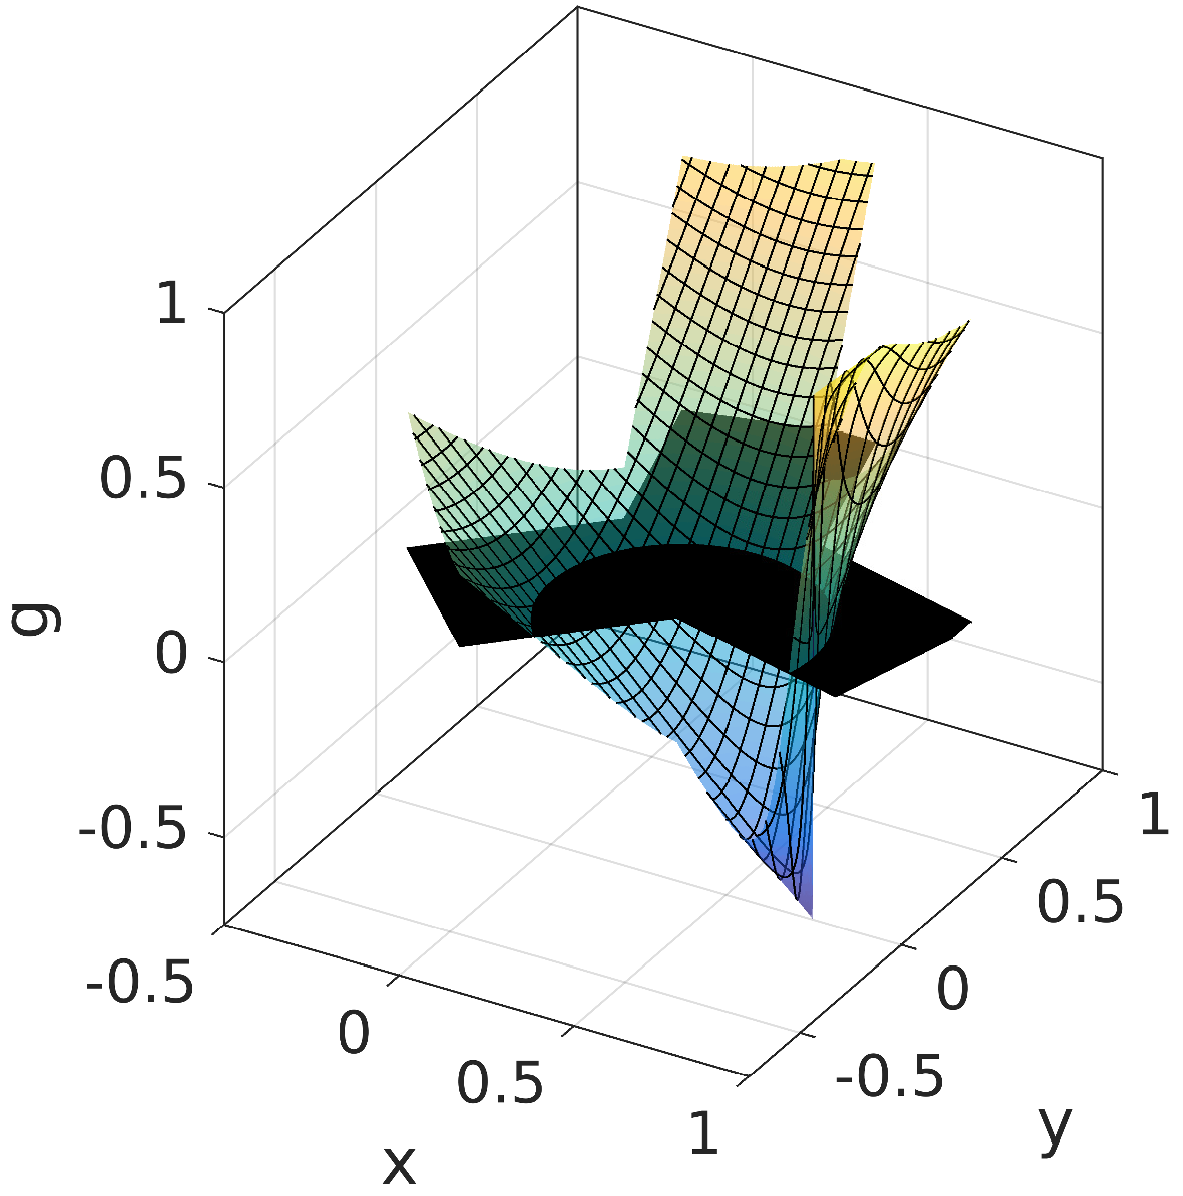
\includegraphics[width=0.24\columnwidth]{fig/moment_hull_2}
  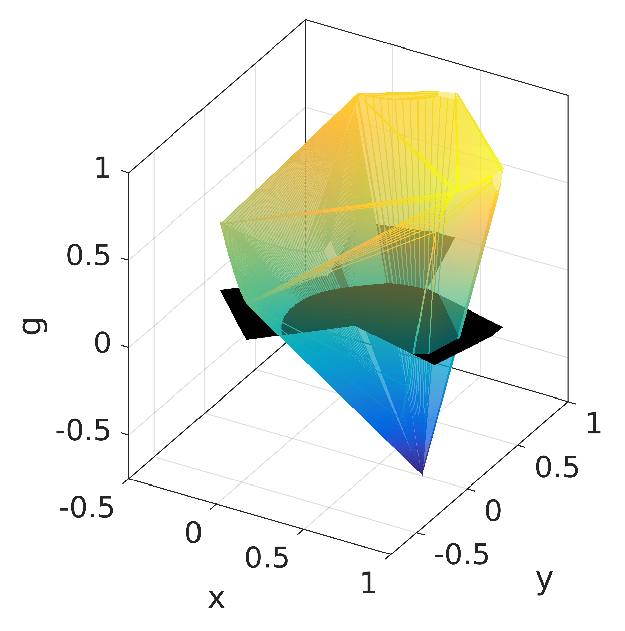
\includegraphics[width=0.24\columnwidth]{fig/moment_hull_3}
  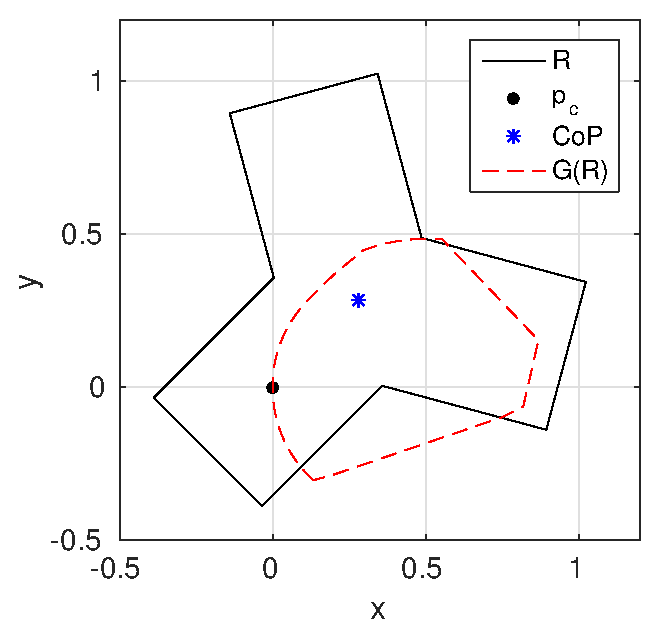
\includegraphics[width=0.24\columnwidth]{fig/CoP_boundary}
  \end{center}
}

\headerbox{Exact Angular Velocity Bounds}{name=ex,column=0,below=bg}{

  Let $\Omega$ be the set of \textbf{feasible} angular velocities
  for a given center of pressure $\mathbf{c}$ and orientation $\rho$.
  \begin{theorem} $\Omega$ is bounded and connected.
  \end{theorem}
  \begin{center}
    \begin{tikzpicture}
      \node[anchor=south west,inner sep=0] (image) at (0,0)
      {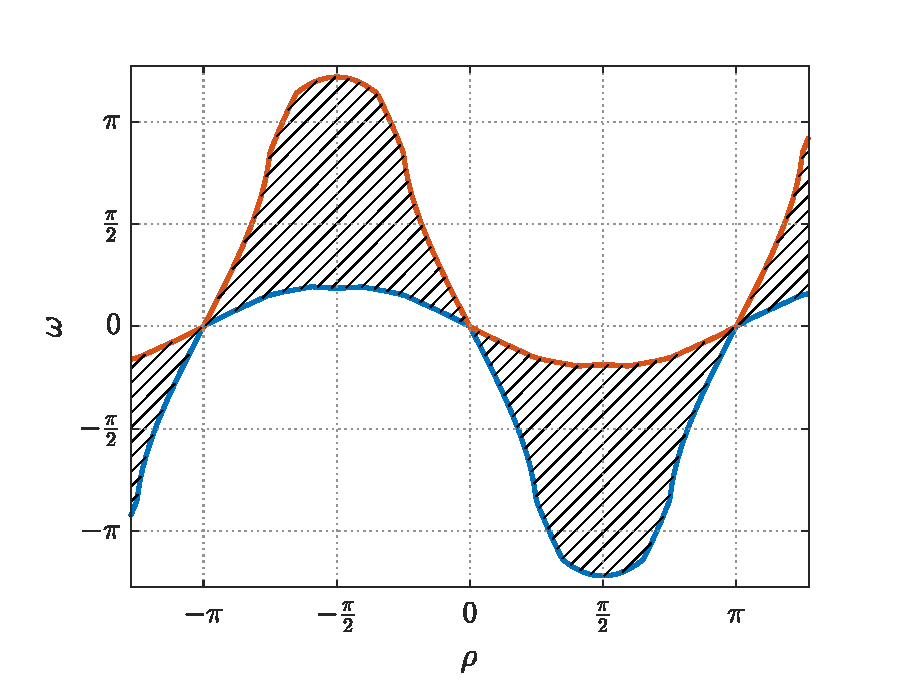
\includegraphics[width=0.7\columnwidth]{fig/omega_bounds_2.eps}};
      \begin{scope}[x={(image.south east)},y={(image.north west)}]
        % \mygrid
        \draw[line width=1.25] (0.425,0.577) -- ++(0,0.275) node[right=3pt] {$\Omega$};
        \definecolor{BLUE}{RGB}{0,113,188}
        \definecolor{ORANGE}{RGB}{216,82,24}
        \draw[line width=1.25,color=BLUE] (0.363,0.373) -- ++(0.03,0) node[right=3pt] {$\beta$};
        \draw[line width=1.25,color=ORANGE] (0.667,0.685) -- ++(0.03,0) node[right=3pt] {$\alpha$};
      \end{scope}
    \end{tikzpicture}
    % {\centering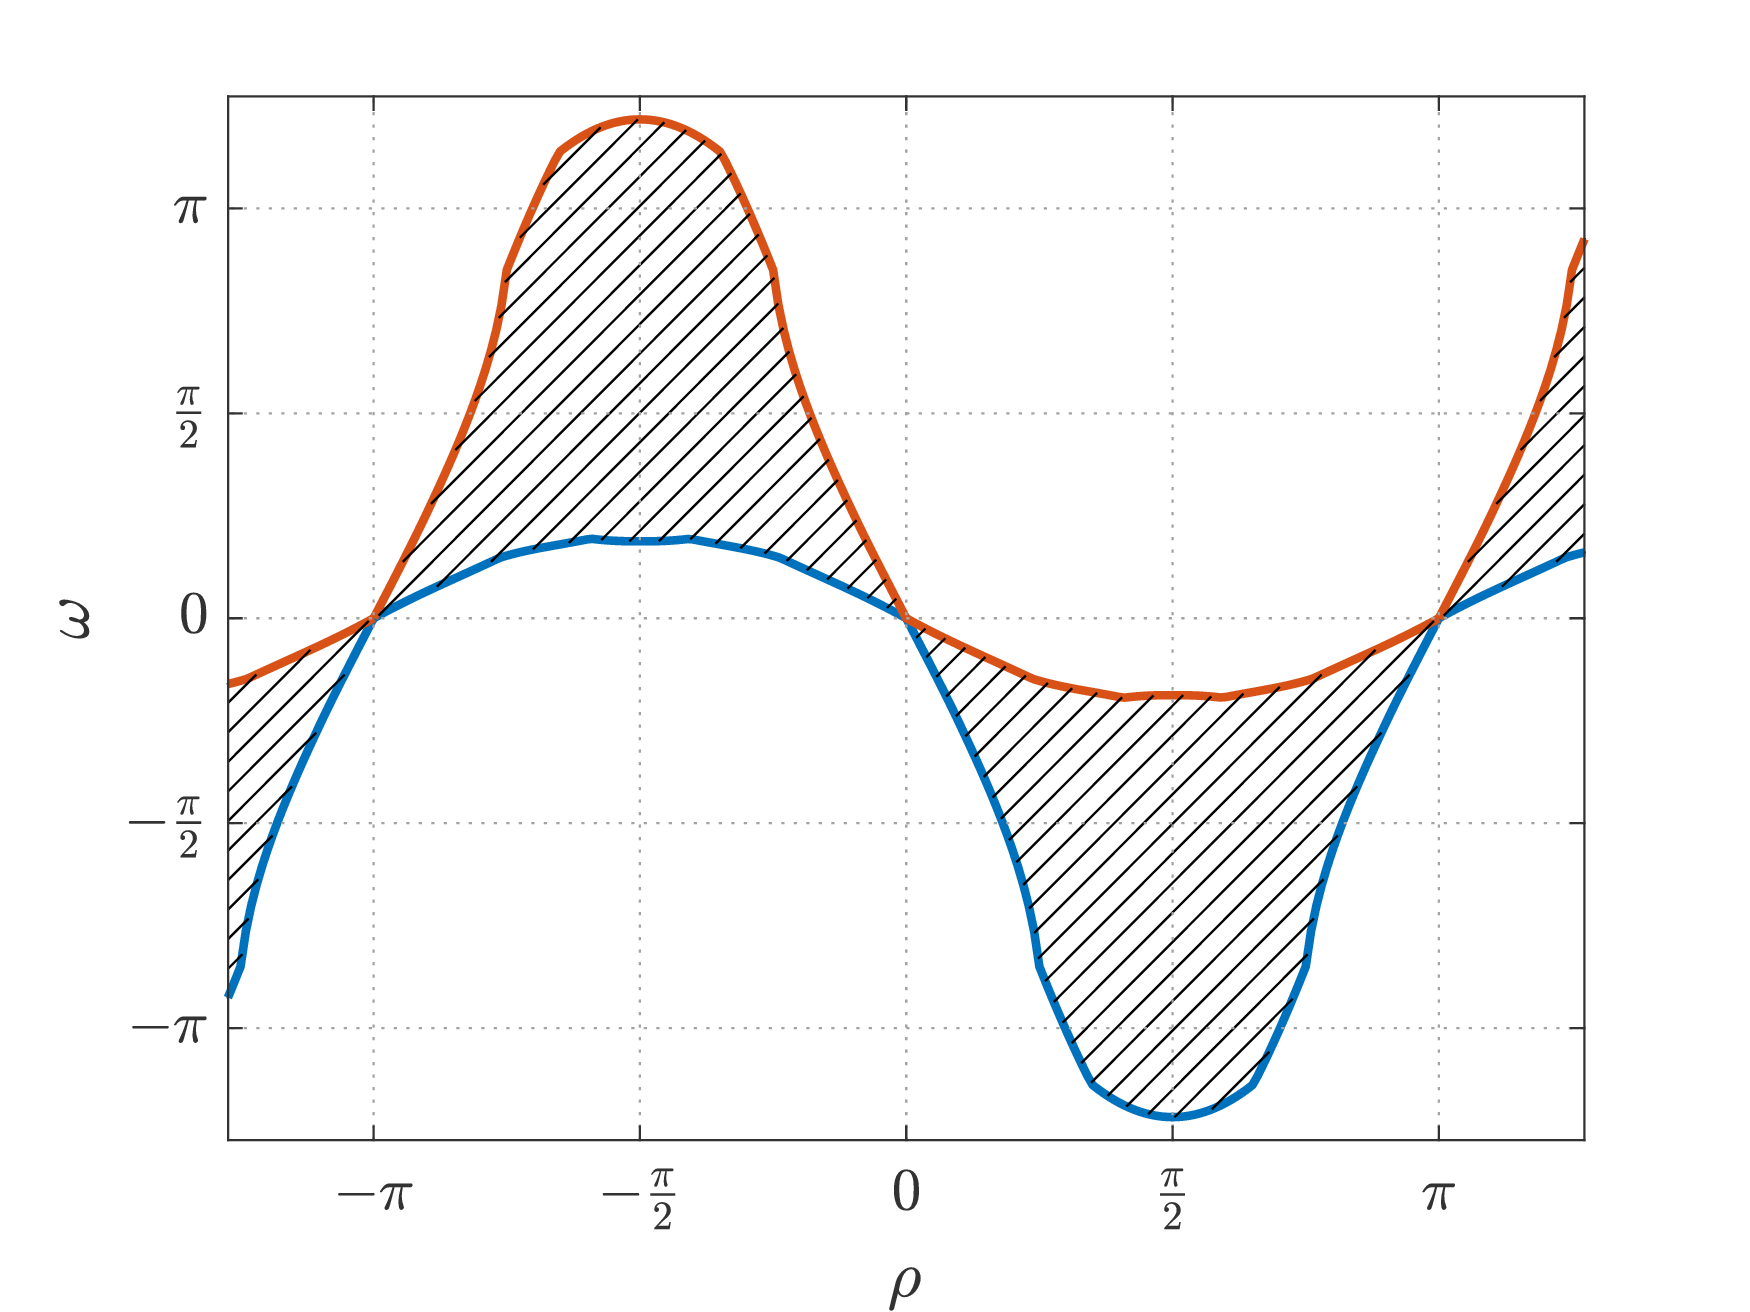
\includegraphics[width=0.5\columnwidth]{fig/omega_bounds_2}}
  \end{center}
  $\therefore$ We can compute $\min\Omega$ and $\max\Omega$ using a
  \textbf{bisection search}.
  \begin{itemize}
  \item $\omega$ is \textbf{feasible} $\Leftrightarrow$ $[\mathbf{c}; 0] \in \conv G(R)$
    % \begin{equation}
    %   \begin{aligned}
    %     & \underset{p}{\text{minimize}}
    %     & & \left\lVert \sum_R -\mu\mathbf{r}\times\frac{\mathbf{v}(\mathbf{r})}{\lVert\mathbf{v}(\mathbf{r})\rVert}p(\mathbf{r})\right\rVert \\
    %     & \text{subject to} 
    %     & & p \in \mathcal{K},
    %   \end{aligned} \label{eq:lin-prog-feasibility}
    % \end{equation}
  \end{itemize}
}
\headerbox{Robotic Pulling Planner}{name=pl,column=1,row=0,}{\vspace{3mm}

  We use Control-limited Differential Dynamic Programming (DDP) to
  plan \textbf{pulling trajectories} that \textbf{guarantee
    convergence} to the final pose \cite{tassa2014control}. 

  \begin{theorem} Pulling has a stable equilibrium at $\rho = 0$. \label{item:1}
  \end{theorem}

  The planner can \textbf{reduce uncertainty} by pulling along the stable direction.\\

  Let $\phi(t)$ be the pulling direction in the global frame. The
  DDP \textbf{dynamics} are given by
  \begin{align}
    \dot{x} &= \cos(\phi(t))\\
    \dot{y} &= \sin(\phi(t))\\
    \dot{u} &=  \alpha(u - \phi(t) + \pi) \label{eq:u-ode}\\ 
    \dot{\ell} &=  \beta(\ell - \phi(t) + \pi).
  \end{align}
  Let $\theta$ be the orientation in the global frame. We can
  \textbf{bound the uncertainty} about $\theta$ using
  \begin{theorem} $l_0 = \theta_0 = u_0 \Rightarrow l(t) \leq \theta(t) \leq u(t)$, $\forall t$,
  \end{theorem}
  $\therefore$ To generate convergent plans, we set the DDP goal to
  \begin{equation}
    \mathbf{x}_F = [x_F, y_F, \theta_F, \theta_F]^T.
  \end{equation}
}

\headerbox{Experiments}{name=exp,column=1,below=pl}{
  \begin{tabular}{@{}cc@{}}
    \multicolumn{1}{m{0.45\columnwidth}}{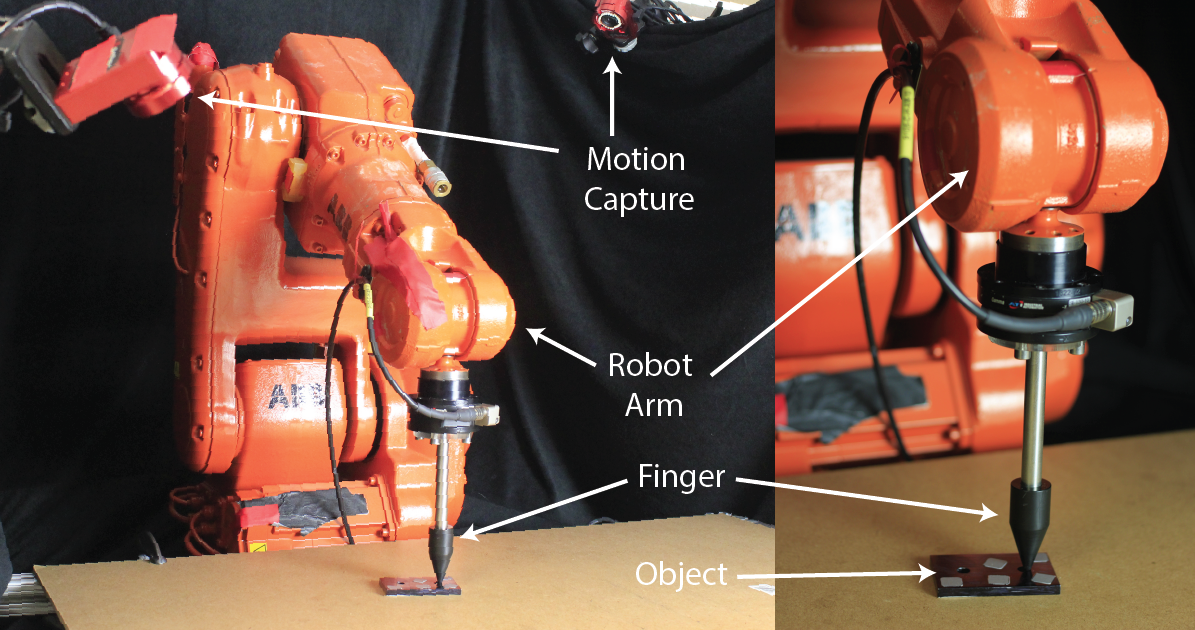
\includegraphics[width=0.5\columnwidth]{fig/hardware.png}} & \multicolumn{1}{m{0.45\columnwidth}}{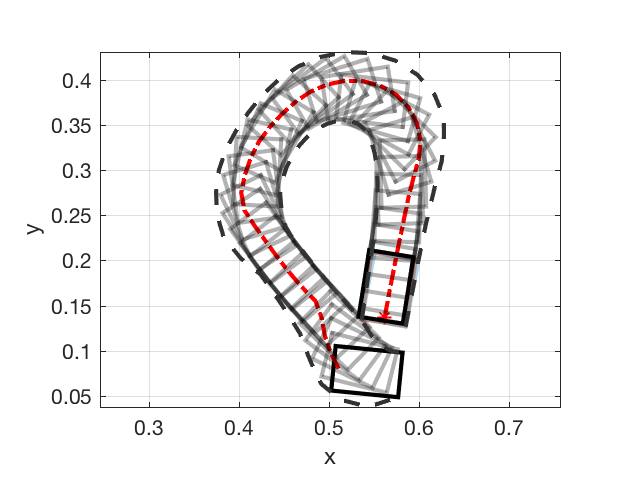
\includegraphics[width=0.5\columnwidth]{fig/trajectory_2.eps}}
     % & 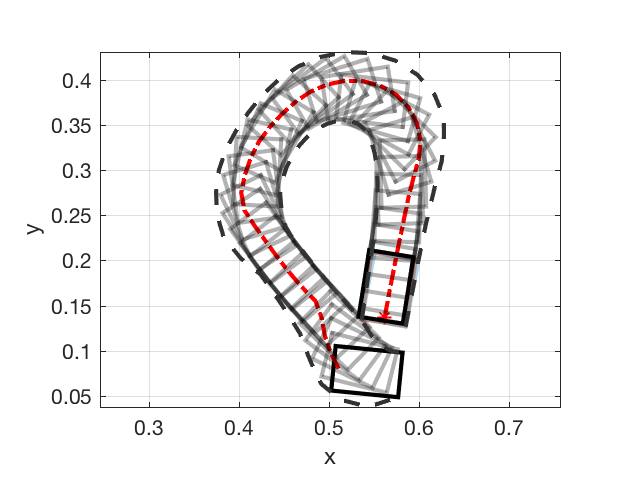
\includegraphics[width=0.5\columnwidth]{fig/trajectory_2.eps}
  \end{tabular}
  We ran 80 trials of robotic pulling to random goal poses. We observed
  \begin{itemize}
  \item Position error: 4.00mm $\pm$ 3.02mm
  \item Angular error: 4.35 degrees $\pm$ 3.14 degrees
  \end{itemize}
  The planner failed 4 times due to the generated trajectory violating
  workspace constraints.

} \headerbox{Future
  work}{name=fw,column=1,below=exp}{
  \begin{itemize}
  \item Apply the exact bounds/planner to real-world robotics problems such as
    NAMO, tabletop rearrangement.
  \end{itemize}
} \headerbox{Conclusion}{name=con,column=1,below=fw}{

  We derived a method for computing \textbf{exact} angular velocity
  bounds and planning convergent pulling trajectories.

  \begin{itemize}
  \item We validated the exact angular velocity bounds on a physical system.
  \item We showed empirically that pulling is a stable method for
    positioning and orienting objects.
  \end{itemize}
}
\headerbox{References}{name=ref,column=1,below=con,bottomaligned=ex}{
  \scriptsize{
    \bibliographystyle{plain}
    \bibliography{references}
  }
}
% \headerbox{Acknowledgements}{name=ack,column=1,below=ref,bottomaligned=ex}{
%   \scriptsize{
%     Eric Huang was supported by the Department of Defense (DoD) through
%     the National Defense Science \& Engineering Graduate Fellowship
%     (NDSEG) Program. This material is based upon work supported by the
%     National Science Foundation under Grants No. IIS1409003 and
%     IIS1637908.
%   }
% }
\end{poster}

\end{document}
